\documentclass[11pt]{article}
%Gummi|061|=)
\usepackage[table]{xcolor} 
\usepackage{vmargin}
\usepackage[T1]{fontenc} %encoding del font
\usepackage[utf8]{inputenc} %encoding dell'input
\usepackage[italian]{babel} %lingua per la formattazione
\usepackage{mparhack}
\usepackage{pgfplotstable}
\usepackage{float}
%pacchetti per la formattazione
\usepackage{calc} %fantasmi

\usepackage{graphicx} %inserire immagini (grafici vettoriali.pdf)
%pacchetti -->\SCfigure \SCtable
\usepackage{booktabs} %pacchetto per per le tabelle
\usepackage{amsmath, amssymb} %pacchetti per usare comandi matematici
\usepackage{pgf,tikz}
\usepackage{caption}
\usepackage{siunitx}
\usepackage{setspace}
\usepackage{subfig}
\usepackage{array}
\usepackage{multirow}


             
\begin{document}

\begin{center}

\textsc{\Huge Esperienza IV}\\[0.5cm]


\large
\title{ESPERIENZA IV}
 
Michele \textsc{Pedrotti}\\
Luigi \textsc{Bassini}\\
Nicola \textsc{Trevisson}\\
Giacomo \textsc{Alberini}

\end{center}


\rowcolors{1}{gray!25}{white}
~\\

\section{Scopo dell'esperienza}
Lo scopo di questa esperienza, è quello di tarare una valvola a spillo. Una valvola a spillo ( o \textit{Fine control needle valve}), è un particolare tipo di valvola che permette di conoscere il flusso di gas in entrata, e risulta estremamente importante in determinati contesti. Il nostro obiettivo sarà proprio quello di misurare il flusso in entrata in una camera di volume (misurato come variazione di pressione in funzione del tempo), al variare del numero di giri di apertura della valvola.
\section{Materiale a disposizione}
\begin{itemize}
\item Impianto da vuoto;
\item Valvola a spillo con regolazione micrometrica;
\item Multimetro e sistema di aquisizione dati;
\item Vacuometro Pirani per la misura della pressione in camera;
\end{itemize}

\section{Taratura della valvola a spillo}
\subsection{Impianto da vuoto}
Per misurare il flusso di gas in entrata nella camera, e quindi tarare la valvola a spillo, è necessario creare il vuoto nella camera. Per raggiungere questo scopo si è utilizzato l'impianto da vuoto già descritto nella relazione precedente. Ne riportiamo di seguito uno schema:
\vspace{-10 pt} 
 \begin{center} 
\begin{figure}[H]
\hspace{-30.5pt}
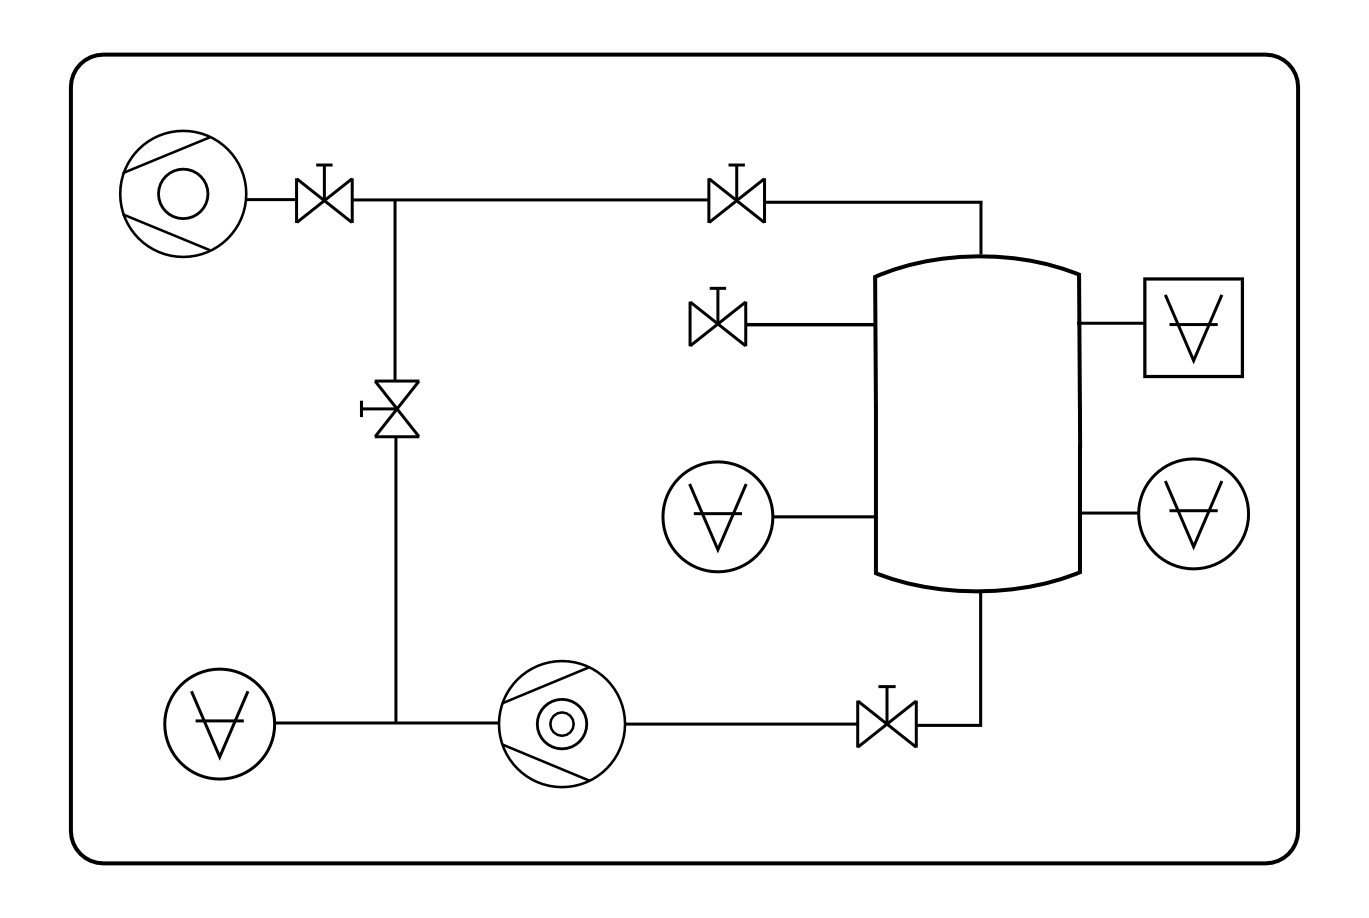
\includegraphics[scale=0.4]{schema_finale.png}
\caption{}
\label{}
\end{figure}
\end{center}

Per prima cosa abbiamo misurato il flusso di gas dovuto alle perdite dell'impianto. Questo flusso dovrà successeivamente essere sottratto alle misure di flusso relative alla valvola a spillo. Per questa prima misura abbiamo raggiunto il vuoto limite del nostro impianto (circa $1.2\cdot10^{-5}$ mbar), e abbiamo quindi misurato la pressione in funzione del tempo utilizzando il software in nostra dotazione.
Successivamente abbiamo creato nuovamente il vuoto limite nella camera (utilizzando le precauzioni dovuto in modo da non danneggiare la pompa turbomolecolare). Durante questo processo abbiamo tenuto completamente aperti i due rubinetti della valvola a spillo (tappando ovviamente l'uscita così da non provocare un repentino riflusso di gas all'interno della camera), così da evitare che si creasse un volume morto nella valvola che avrebbe poi pesantemente inciso sui primi dati acquisiti. Raggiunto il vuoto limite abbiamo sigillato la camera (tenendo accesa la pompa turbomolecolare),calibrata la valvola a spillo sulla prima tacca e quindi tolto il tappo all'uscita della valvola. Con il software abbiamo quindi acquisito i dati Pressione-Tempo. 
A questo proposito è rilevante notare che le misure acquisite in entrata dal software sono relative al voltaggio rilevato dal Pirani. Questo comporta due importanti situazioni. Prima di tutto il range del Pirani va da $10^{-3}$ mbar a 10 mbar, quindi le misure di pressioni inferiori o superiori a questi valori non possono essere considerate attendibili. Inoltre il Pirani lavora attraverso diverse conversioni, e per questo l'incertezza sulle misure di pressione è molto elevata, dell'ordine del 5\%\ in termini di errore relativo. 
Una volta acquisiti i dati è necessario ripetere l'intera sequenza aprendo questa volta la volvola di due tacche. L'operazione è stata ripetuta otto volte, fino ad aprire la valvola all'ottava tacca.  

\end{document} 